%  template.tex for Biometrics papers
%
%  This file provides a template for Biometrics authors.  Use this
%  template as the starting point for creating your manuscript document.
%  See the file biomsample.tex for an example of a full-blown manuscript.

%  ALWAYS USE THE referee OPTION WITH PAPERS SUBMITTED TO BIOMETRICS!!!
%  You can see what your paper would look like typeset by removing
%  the referee option.  Because the typeset version will be in two
%  columns, however, some of your equations may be too long. DO NOT
%  use the \longequation option discussed in the user guide!!!  This option
%  is reserved ONLY for equations that are impossible to split across 
%  multiple lines; e.g., a very wide matrix.  Instead, type your equations 
%  so that they stay in one column and are split across several lines, 
%  as are almost all equations in the journal.  Use a recent version of the
%  journal as a guide. 
%  
\documentclass[useAMS,usenatbib,referee]{biom}
%\documentclass[useAMS,usenatbib]{biom}
\usepackage{graphicx}
\usepackage{amsmath,amsfonts}
\usepackage{xcolor}
%\renewcommand\thesection{\Alph{section}}
%\renewcommand\thesubsection{\thesection.\arabic{subsection}}
%\usepackage{amssymb}
%documentclass[useAMS]{biom}
%
%  If your system does not have the AMS fonts version 2.0 installed, then
%  remove the useAMS option.
%
%  useAMS allows you to obtain upright Greek characters.
%  e.g. \umu, \upi etc.  See the section on "Upright Greek characters" in
%  this guide for further information.
%
%  If you are using AMS 2.0 fonts, bold math letters/symbols are available
%  at a larger range of sizes for NFSS release 1 and 2 (using \boldmath or
%  preferably \bmath).
% 
%  Other options are described in the user guide. Here are a few:
% 
%  -  If you use Patrick Daly's natbib  to cross-reference your 
%     bibliography entries, use the usenatbib option
%
%  -  If you use \includegraphics (graphicx package) for importing graphics
%     into your figures, use the usegraphicx option
% 
%  If you wish to typeset the paper in Times font (if you do not have the
%  PostScript Type 1 Computer Modern fonts you will need to do this to get
%  smoother fonts in a PDF file) then uncomment the next line
%  \usepackage{Times}

%%%%% PLACE YOUR OWN MACROS HERE %%%%%

\def\bSig\bmath{\Sigma}
\newcommand{\VS}{V\&S}
\newcommand{\tr}{\mbox{tr}}
\newcommand{\tcr}[1]{\textcolor{red}{#1}}
\newcommand{\tcb}[1]{\textcolor{blue}{#1}}
\newcommand{\tco}[1]{\textcolor{orange}{#1}}
%  The rotating package allows you to have tables displayed in landscape
%  mode.  The rotating package is NOT included in this distribution, but
%  can be obtained from the CTAN archive.  USE OF LANDSCAPE TABLES IS
%  STRONGLY DISCOURAGED -- create landscape tables only as a last resort if
%  you see no other way to display the information.  If you do this,
%  then you need the following command.

%\usepackage[figuresright]{rotating}

%%%%%%%%%%%%%%%%%%%%%%%%%%%%%%%%%%%%%%%%%%%%%%%%%%%%%%%%%%%%%%%%%%%%%

%  Here, place your title and author information.  Note that in 
%  use of the \author command, you create your own footnotes.  Follow
%  the examples below in creating your author and affiliation information.
%  Also consult a recent issue of the journal for examples of formatting.

%\title{A Structured Framework for Bayesian Sequential Monitoring in Clinical Trials}

%  Here are examples of different configurations of author/affiliation
%  displays.  According to the Biometrics style, in some instances,
%  the convention is to have superscript *, **, etc footnotes to indicate 
%  which of multiple email addresses belong to which author.  In this case,
%  use the \email{ } command to produce the emails in the display.

%  In other cases, such as a single author or two authors from 
%  different institutions, there should be no footnoting.  Here, use
%  the \emailx{ } command instead. 

%  The examples below correspond to almost every possible configuration
%  of authors and may be used as a guide.  For other configurations, consult
%  a recent issue of the journal.

%  Single author -- USE \emailx{ } here so that no asterisk footnoting
%  for the email address will be produced.

%\author{John Author\emailx{email@address.edu} \\
%Department of Statistics, University of Warwick, Coventry CV4 7AL, U.K.}

%  Two authors from the same institution, with both emails -- use
%  \email{ } here to produce the asterisk footnoting for each email address

%\author{John Author$^{*}$\email{author@address.edu} and
%Kathy Authoress$^{**}$\email{email2@address.edu} \\
%Department of Statistics, University of Warwick, Coventry CV4 7AL, U.K.}

%  Exactly two authors from different institutions, with both emails  
%  USE \emailx{ } here so that no asterisk footnoting for the email address
%  is produced.

%\author
%{John Author\emailx{author@address.edu} \\
%Department of Statistics, University of Warwick, Coventry CV4 7AL, U.K. 
%\and
%Kathy Author\emailx{anotherauthor@address.edu} \\
%Department of Biostatistics, University of North Carolina at Chapel Hill, 
%Chapel Hill, North Carolina, U.S.A.}

%  Three or more authors from same institution with all emails displayed
%  and footnoted using asterisks -- use \email{ } 

%\author{John Author$^*$\email{author@address.edu}, 
%Jane Author$^{**}$\email{jane@address.edu}, and 
%Dick Author$^{***}$\email{dick@address.edu} \\
%Department of Statistics, University of Warwick, Coventry CV4 7AL, U.K}

%  Three or more authors from same institution with one corresponding email
%  displayed

%\author{John Author$^*$\email{author@address.edu}, 
%Jane Author, and Dick Author \\
%Department of Statistics, University of Warwick, Coventry CV4 7AL, U.K}

%  Three or more authors, with at least two different institutions,
%  more than one email displayed 

%\author{John Author$^{1,*}$\email{author@address.edu}, 
%Kathy Author$^{2,**}$\email{anotherauthor@address.edu}, and 
%Wilma Flinstone$^{3,***}$\email{wilma@bedrock.edu} \\
%$^{1}$Department of Statistics, University of Warwick, Coventry CV4 7AL, U.K \\
%$^{2}$Department of Biostatistics, University of North Carolina at 
%Chapel Hill, Chapel Hill, North Carolina, U.S.A. \\
%$^{3}$Department of Geology, University of Bedrock, Bedrock, Kansas, U.S.A.}

%  Three or more authors with at least two different institutions and only
%  one email displayed

\author{Evan Kwiatkowski$^{1,*}$\email{ekwiatkowski@unc.edu}, 
Eugenio Andraca-Carrera$^{2}$, Mat Soukup$^{2}$, and Matthew A. Psioda$^{1}$ \\
$^{1}$Department of Biostatistics, University of North Carolina, \\
McGavran-Greenberg Hall, CB\#7420, \\
Chapel Hill, North Carolina, USA\\
$^{2}$Division of Biometrics VII, Office of Biostatistics, \\
Center for Drug Evaluation and Research, US Food and Drug Administration, \\
Silver Spring, Maryland, USA}

\DeclareMathOperator*{\argmax}{arg\,max}
\DeclareMathOperator*{\argmin}{arg\,min}

\begin{document}


%section*{Supplementary Material}

\section*{Web Appendix A: Bayesian Hypothesis Testing}\label{sec:hypothesis}
Consider the hypotheses $H_0:\theta\in\Theta_{0}$ versus $H_1:\theta\in\Theta_{1}$ where $\Theta_{0}\bigcup \Theta_{1} = \Theta$ and $\Theta_{0} \bigcap \Theta_{1} = \emptyset$.
%
Formal Bayesian hypothesis testing requires the specification of prior probabilities on the hypotheses (e.g., $p(H_i)$ for $i=0,1$)
and prior distributions for $\left(\theta,\eta\right)$ specified over the parameter space defined with respect to each of the 
hypotheses (e.g. $\pi\left(\theta,\eta \big| H_i\right)$ for $i=0,1$). 
%

The posterior probability of hypothesis $H_i$ is given by 
\begin{equation}\label{eq:equation1}
p(H_i|\bmath{D})=\frac{p(\bmath{D}|H_i)\cdot p(H_i)}{p(\bmath{D}|H_0)\cdot p(H_0)+p(\bmath{D}|H_1)\cdot p(H_1)},
\end{equation}
where $p(\bmath{D}|H_i) = \int_{\Theta_i} p(\bmath{D}|\theta)\pi(\theta|H_i)d\theta$ is the marginal likelihood associated with hypothesis $H_i$.
%
In practice, most Bayesian methods for clinical trials perform hypothesis testing based on the posterior probability of the \textit{event defining $H_i$}.
%
For this approach, one simply needs to specify a prior $\pi\left(\theta\right)$ representing belief about $\theta$ overall and compute the posterior distribution.
%
The posterior probability that $\theta\in\Theta_i$ is given by
\begin{equation}\label{eq:equation2}
P(\theta\in\Theta_i|\bmath{D})
%=\frac{\int_{\Theta_i} p(\bmath{D}|\theta)\pi (\theta)d\theta}{\int_{\Theta}p(\bmath{D}|\theta)\pi(\theta) d\theta}
=\frac{\int_{\Theta_i} p(\bmath{D}|\theta)\pi (\theta|\theta\in\Theta_i)d\theta\cdot P(\theta\in\Theta_i)}
      { \sum_{j=0,1} \int_{\Theta_j}p(\bmath{D}|\theta)\pi (\theta|\theta\in\Theta_j)d\theta\cdot P(\theta\in\Theta_j) }
\end{equation}
where $P(\theta\in\Theta_i)=\int_{\Theta_i}\pi(\theta)d\theta$. 
%
We can readily see that the $P(\theta\in\Theta_i|\bmath{D})$ is equal to $p(H_i|\bmath{D})$ if one takes
$p(H_i) =P(\theta\in\Theta_i)$ and $\pi\left(\theta \big| H_i\right) = \pi\left(\theta\big|\theta \in \Theta_i\right)$ for $i=0,1$.
%
If in fact $\pi\left(\theta\right)$ does represent belief about $\theta$, these choices are perhaps the most intuitive and thus 
we should have no reservation referring to $P(\theta\in\Theta_i|\bmath{D})$ as the probability that hypothesis $H_i$ is true.
\section*{Web Appendix B: Monitoring Prior Parameterization}\label{sec:gen_normal_details}

\subsubsection*{Normal Distribution $\mathcal{N}_p(\tilde{\mu},q)$}\label{sec:normal_tail_area}
%The specification of the mean and variance of a normal distribution completely specifies the mode value and a tail-probability constraint, and is therefore sufficient for defining enthusiastic and skeptical priors.

Suppose $\theta\sim\mathcal{N}(\mu,\sigma)$ is a normal random variable that satisfies $\rmn{mode}(\theta)=\tilde{\mu}$ and $P(\theta\leq q)=p$. The values for the mean and standard deviation are $\mu=\tilde{\mu}$ and $\sigma=\frac{q-\mu}{\Phi^{-1}(p)}$, where $\Phi$ denotes the cumulative distribution function for a standard normal distribution and $\Phi^{-1}$ denotes its quantile function. Therefore we can denote the distribution with the desired mode and tail probability constraint as  $\theta\sim\mathcal{N}_p(\tilde{\mu},q)$, which is well-defined for values $(\mu,q,p)$ that satisfy $\frac{q-\mu}{p-0.5}>0$. Since the normal distribution is completely specified by $(\mu, \sigma)$, quantities such as $P(\theta\leq\tilde{q})$ are also specified for any $\tilde{q}\in\mathbb{R}$. In particular, if $\theta\sim\mathcal{N}_p(\tilde{\mu},q)$ then $P(\theta\leq\frac{q+\mu}{2})=\Phi(\frac{\Phi^{-1}(p)}{2})$. Furthermore, $P(\theta\in(\mu,\frac{q+\mu}{2}))=|p-\Phi(\frac{\Phi^{-1}(p)}{2})|$. 

\subsubsection*{Generalized Normal Distributions $\mathcal{GN}_p(\tilde{\mu},q,\gamma)$}\label{sec:gen_norm_appendix}
Let $F_{\mu,\alpha,\beta}$ denote the cumulative distribution function of $\mathcal{GN}(\mu,\alpha,\beta)$. The CDF of a generalized normal random variable $\theta\sim\mathcal{GN}(\mu,\alpha,\beta)$ can be expressed as \citep{Griffin2018}
\begin{equation}
P(\theta\leq q|\mu,\alpha,\beta)=\frac{1}{2}+\frac{\rmn{sign}(q-\mu)}{2}\int_0^{|q-\mu|^\beta}\frac{w^{1/\beta-1}}{\alpha\Gamma(1/\beta)}\rmn{exp}\left\{-\left(\frac{1}{\alpha}\right)^\beta w\right\} dw
\end{equation}
%Computations involving $F_{\mu,\alpha,\beta}$ are done using the gnorm package \citep{Griffin2018}. 
Define $\theta\sim\mathcal{GN}_p(\tilde{\mu},q,\gamma)$ as the generalized normal distribution $\mathcal{GN}(\mu,\alpha,\beta)$ that satisfies mode$(\theta)=\tilde{\mu}$, $P(\theta\leq q)=p$, and $P(\theta\in(q,\frac{q+\mu}{2}))=\gamma\cdot|p-\Phi(\frac{\Phi^{-1}(p)}{2})|$.
%\end{mydef}
%
The mode is equal to $\mu=\tilde{\mu}$, and $\alpha$ and $\beta$ are determined to minimize the function $(F_{\mu,\alpha,\beta}(q)-p)^2+(F_{\mu,\alpha,\beta}(\frac{q+\mu}{2})-\gamma\cdot|p-\Phi(\frac{\Phi^{-1}(p)}{2})|)^2$ with box-constrained optimization \citep{Byrd1995}. %The restrictions on well-defined choices of $(p,\tilde{\mu},q,\gamma)$ for the $\theta\sim\mathcal{GN}_p(\tilde{\mu},q,\gamma)$ distribution are described in the appendix.

Using this notation to define the distributions in Figure \ref{fig:figure1} yields the default enthusiastic prior as $\mathcal{GN}_{p=0.025}(\tilde{\mu}=\theta_1,q=\theta_0,\gamma=1)$, the concentrated enthusiastic prior as $\mathcal{GN}_{p=0.025}(\tilde{\mu}=\theta_1,q=\theta_0,\gamma=0.75)$, the flattened enthusiastic prior as $\mathcal{GN}_{p=0.025}(\tilde{\mu}=\theta_1,q=\theta_0,\gamma=1.5)$, and the locally non-informative prior as $\mathcal{GN}_{p=0.025}(\tilde{\mu}=\frac{\theta_0+\theta_1}{2},q=\frac{3\theta_0-\theta_1}{2},\gamma=1.5)$.
\subsubsection*{Truncated Generalized Normal Distribution $\mathcal{GN}_{p,\Theta}(\tilde{\mu},q,\gamma)$}\label{sec:gen_normal_appendix}
The density for a generalized normal distribution truncated to the interval domain $\Theta=(\theta_{min},\theta_{max})$, denoted by $\mathcal{GN}_\Theta(\mu,\alpha,\beta)$, is $f(\theta)=c\cdot\exp\left\{-\frac{|\theta-\mu|}{\alpha}^{\beta}\right\}{I(\theta\in \Theta)}$ where $c=\frac{\beta}{2\alpha \Gamma(1/\beta)}({F_{\mu,\alpha,\beta}(\theta_{max})-F_{\mu,\alpha,\beta}(\theta_{min})})^{-1}$. 
%\begin{mydef}\label{def:gennormaltruncated}
Define $\theta\sim\mathcal{GN}_{p,\Theta}(\tilde{\mu},q,\gamma)$ as the truncated generalized normal distribution $\mathcal{GN}_\Theta(\mu,\alpha,\beta)$ that satisfies mode$(\theta)=\tilde{\mu}$, $P(\theta\leq q)=p$, and $P(\theta\in(q,\frac{q+\mu}{2}))=\gamma|p-\Phi(\frac{\Phi^{-1}(p)}{2})|$.

Using this notation to define the distribution in Figure \ref{fig:figure5} yields the joint distribution $\pi(\theta,\eta)=\pi(\theta)\times\pi(\eta|\theta)$, as $
\pi(\theta)\sim\mathcal{GN}_{p=0.975,\Theta=[-1,1]}(\tilde{\mu}=\theta_0,q=\theta_1,\gamma=1)$ and $\pi(\eta|\theta)\sim \mathcal{GN}_{p=0.975,\Theta=[\rmn{max}(-\theta,0),\rmn{min}(1,1+\theta)]}(\tilde{\mu}=\eta_0,q=\eta_1,\gamma=1)$.

%\end{mydef}
%
%\subsection{Parameterizing the $\mathcal{GN}_p(\tilde{\mu},q,\gamma)$ Distribution}
%The restrictions on the choice of $(p,\tilde{\mu},q,\gamma)$ for the $\theta\sim\mathcal{GN}_p(\tilde{\mu},q,\gamma)$ distribution to be well-defined:

\section*{Web Appendix C: Type 1 Error Rate Depending on Enrollment Schemes}
Recall Figure \ref{fig:ex1t1e} from Section \ref{sec:example1} which showed Type 1 error properties for the single-arm design. Figure \ref{fig:ex1t1e_longer} shows results from a design that has a longer follow-up period. The interim sample sizes are the same for each monitoring frequency, however, the final sample sizes under the longer follow-up designs are much larger (over 20 patients in follow-up for monitoring frequencies of 8 or fewer, compared to approximately 6 patients in the shorter follow-up designs). The final probability of efficacy criteria being satisfied is generally slightly lower in the longer follow-up design, which is what we would expect since the larger final sample size contains more data consistent with a null result.
\begin{figure}\begin{center}

   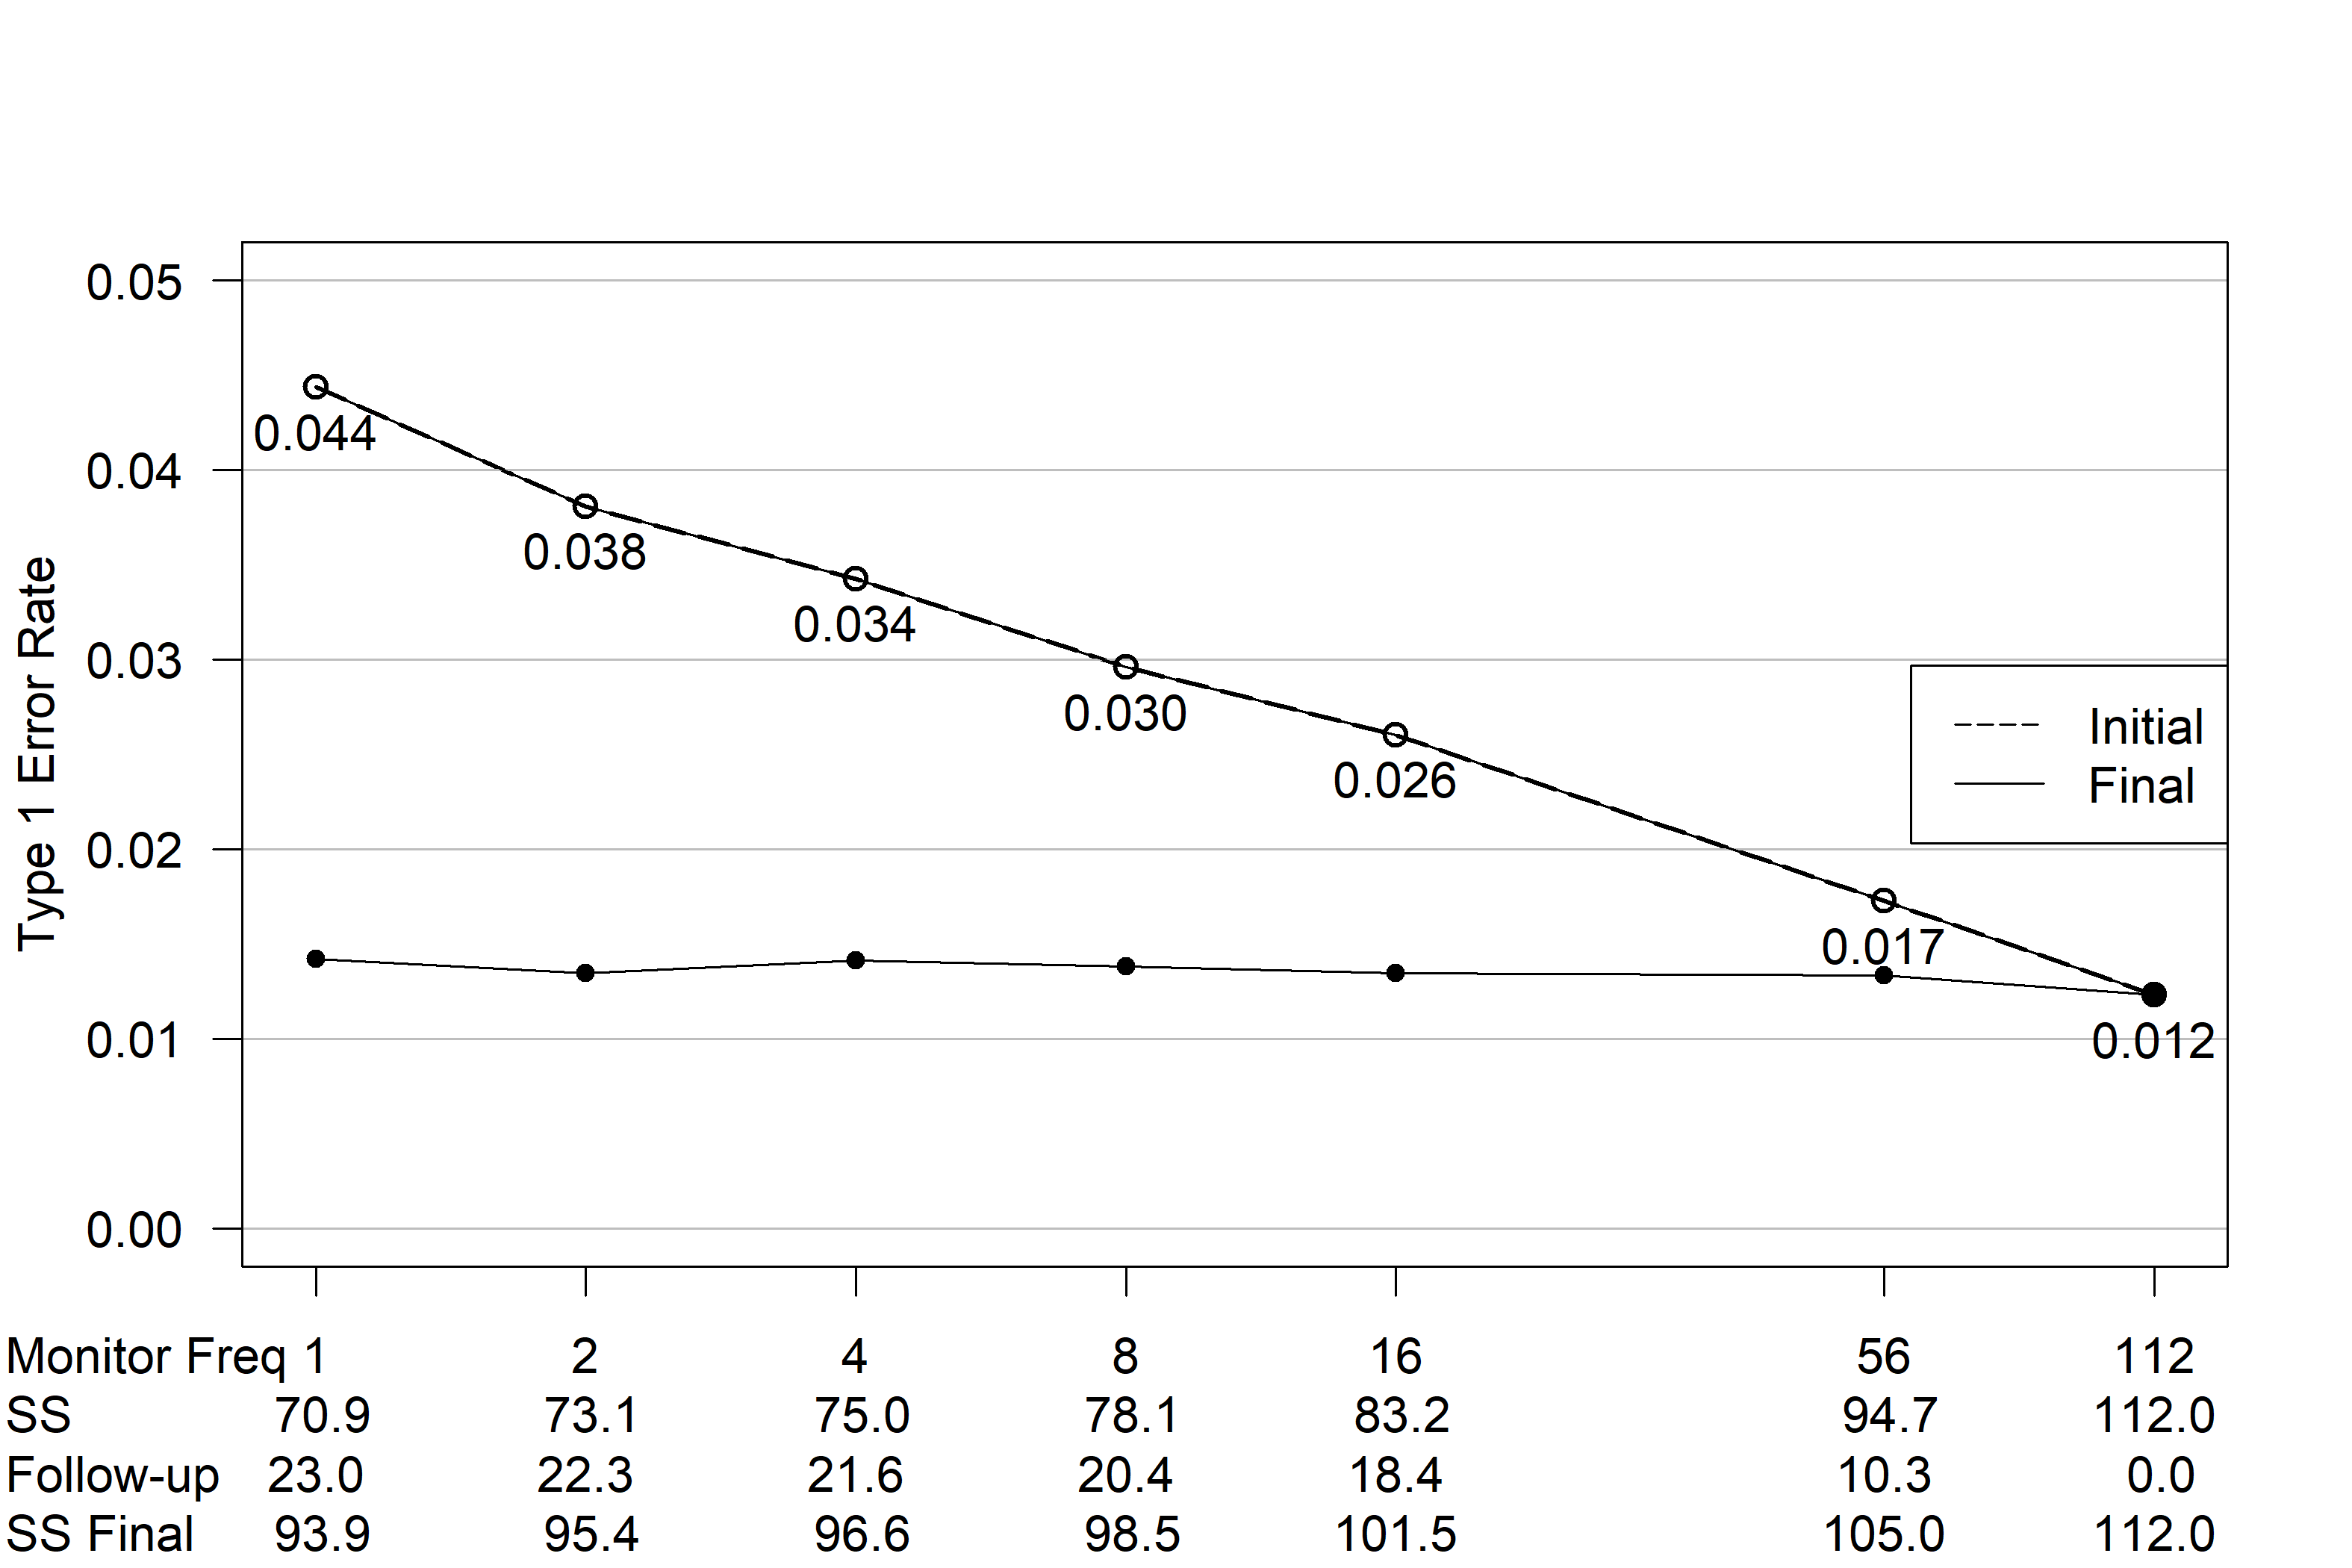
\includegraphics[width=6in]{figureS1.png}
    \caption{Single arm design from Example \ref{sec:example1} with a longer follow-up period. Probability of efficacy criteria being satisfied when $\theta=\theta_0$. SS; sample size. Monitor Freq; monitoring frequency.}
	\label{fig:ex1t1e_longer}

\end{center}
\end{figure}
\section*{Web Appendix D: Robustness of Parameterizations of Monitoring Priors}\label{sec:priorRobustness}
The analyses done in Section \ref{sec:example1} used a concentrated skeptical prior and default enthusiastic prior. In this section we show the four possible designs using the combinations of skeptical and enthusiastic prior given in Figure \ref{fig:figure1}.

Figures \ref{fig:robustness1}-\ref{fig:robustness2} shows what happens when the enthusiastic prior shifts from default to flattened, with the skeptical prior remaining fixed. Note that in the region between $\theta_0$ and $\frac{\theta_0+\theta_1}{2}$ as the enthusiastic prior shifts from default to flattened, (a) the probability of stopping early for futility increases (b) the probability of inconclusive findings decreases and (c) the intermediate and final sample sizes decrease. This is because the enthusiastic prior gives more mass in for this region of $\theta$. The flattened enthusiastic prior was used in Section \ref{sec:example1} to enhance the ability of futility monitoring to reduce the sample size.

Contrasting \ref{fig:robustness1} and \ref{fig:robustness2}, we see that the probability of stopping early for efficacy is much higher at $\theta_0$ when the default skeptical prior is used rather than the concentrated skeptical prior. This is because the default skeptical prior has less mass around $\theta=\theta_0$, therefore it is easier to convince the skeptic that $\theta>\theta_0$ under the null result $\theta=\theta_0$. The concentrated skeptical prior was used in Section \ref{sec:example1} to limit this probability and provide better Type 1 error control.

The choice of skeptical and enthusiastic prior affects the analysis, and their specification (e.g. default, skeptical, enthusiastic) should be made with these properties in mind.

\begin{figure}\begin{center}

 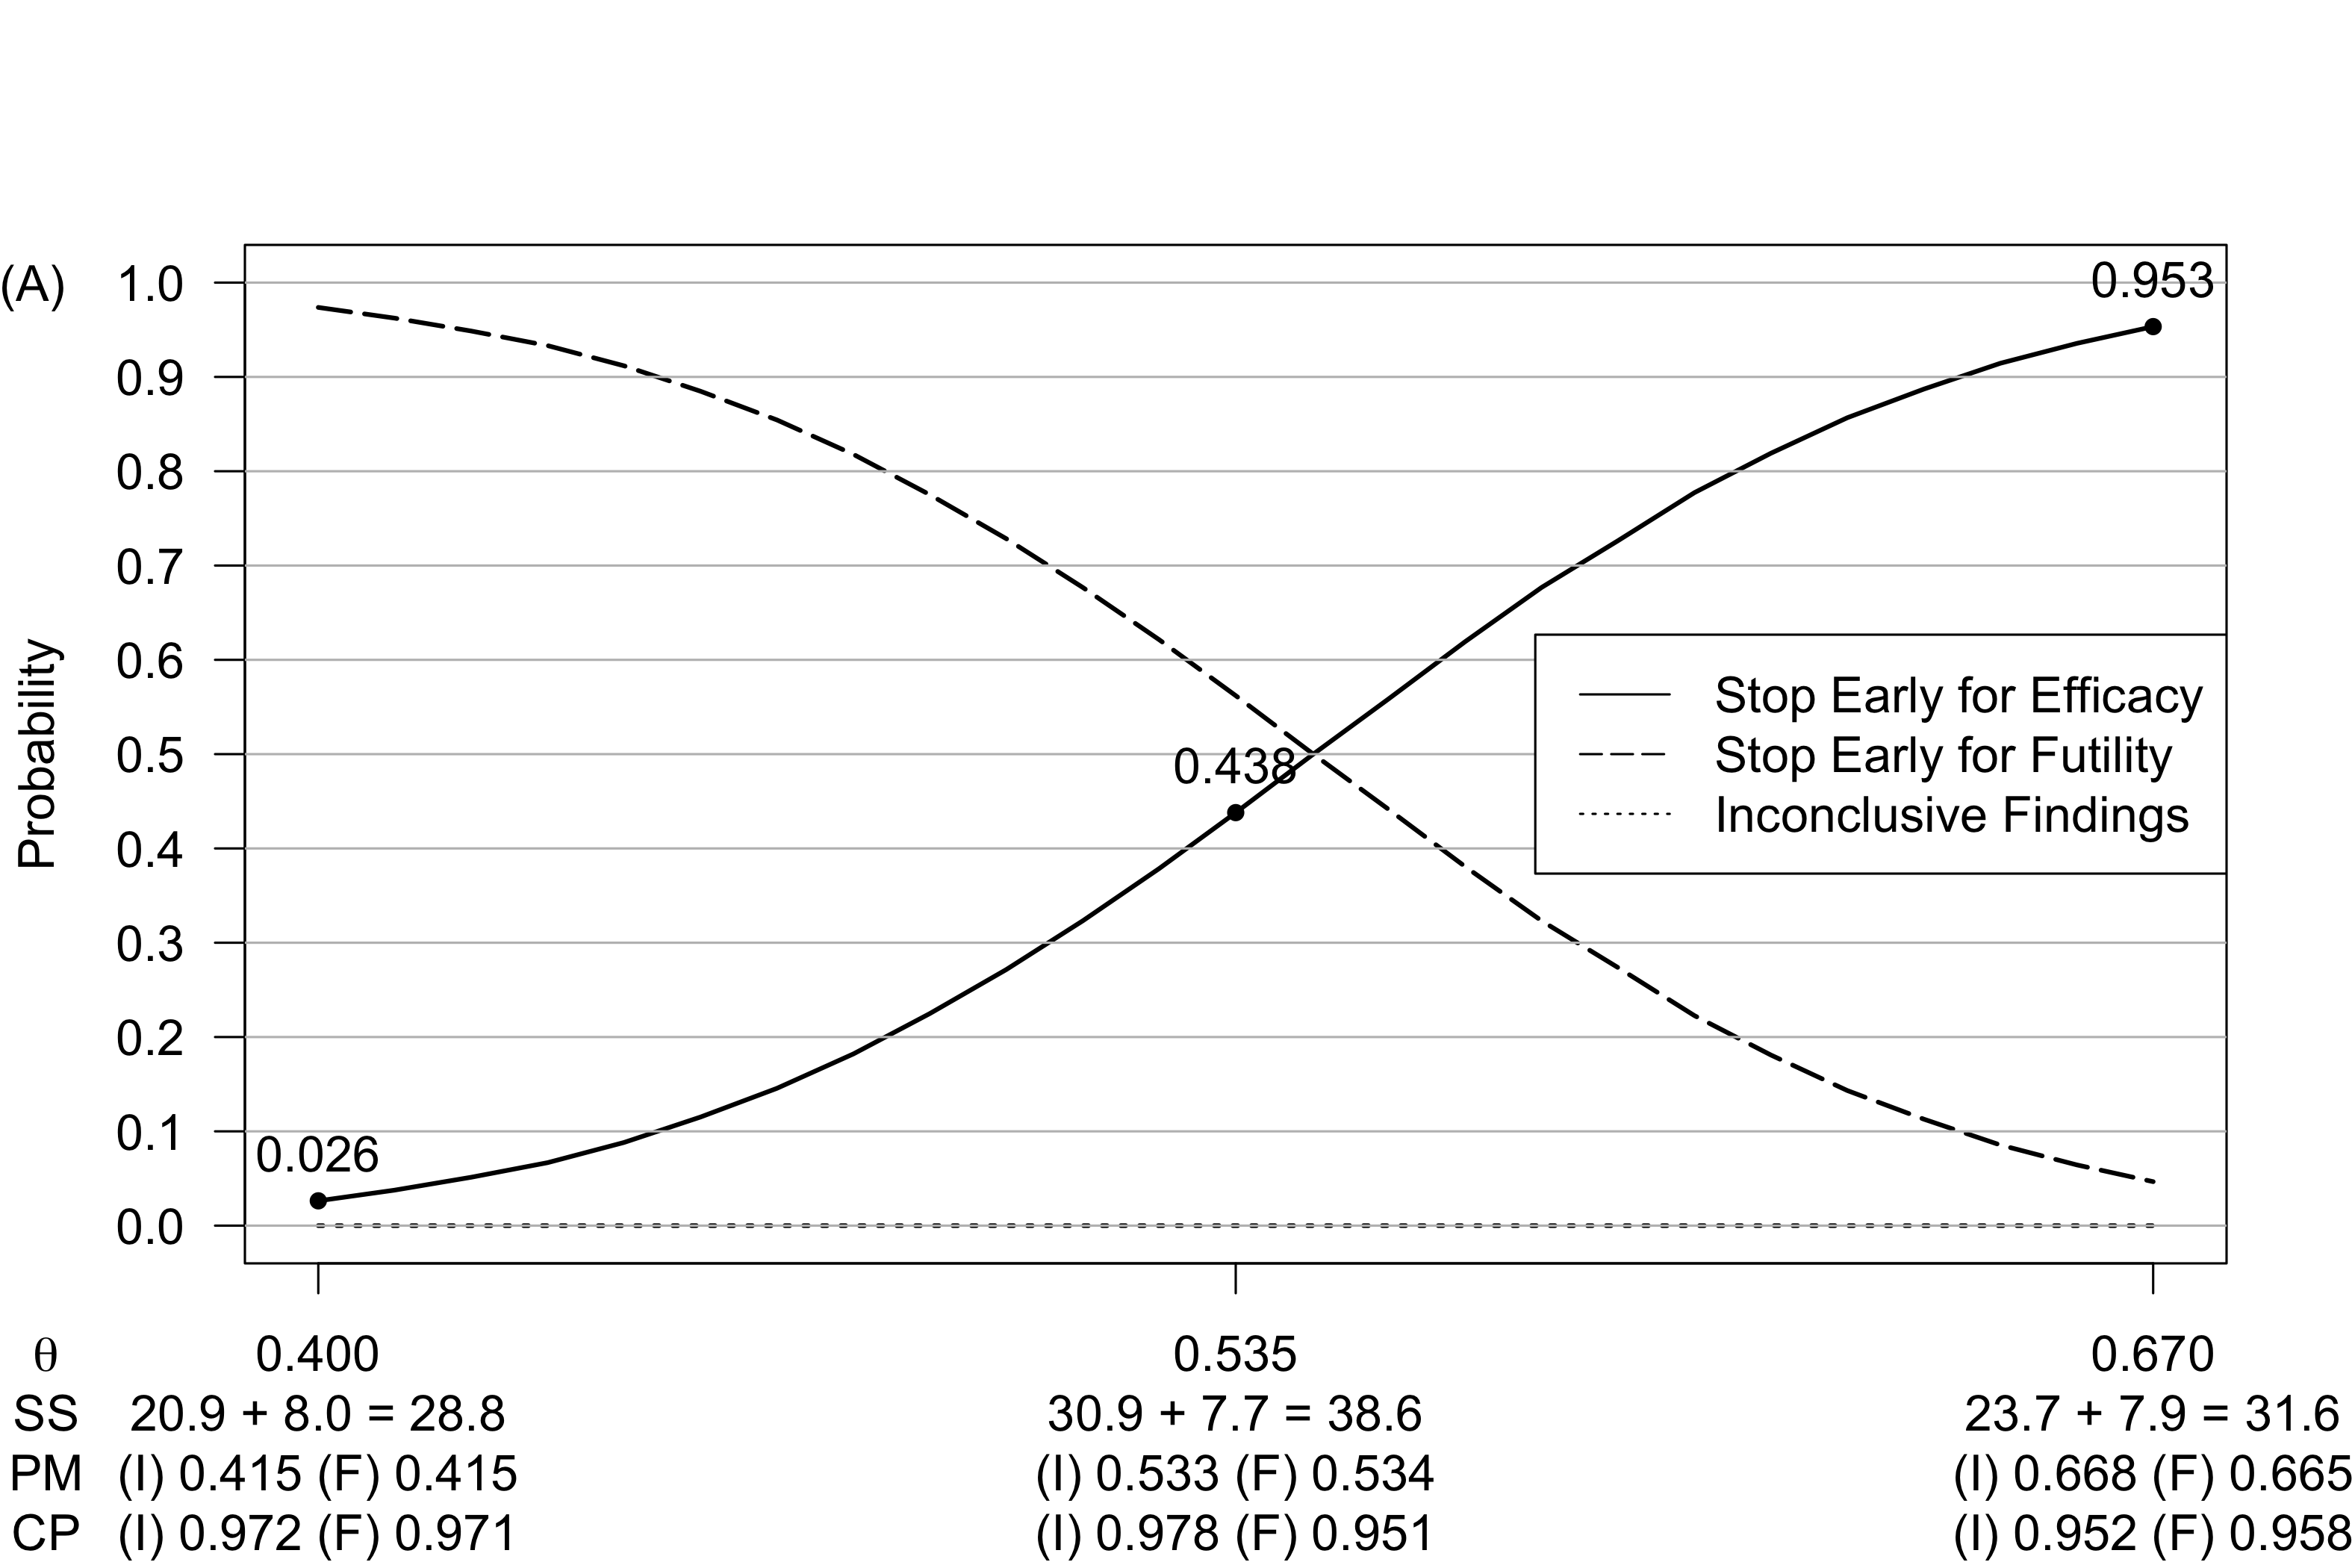
\includegraphics[width=6in]{figureS2a.png}
 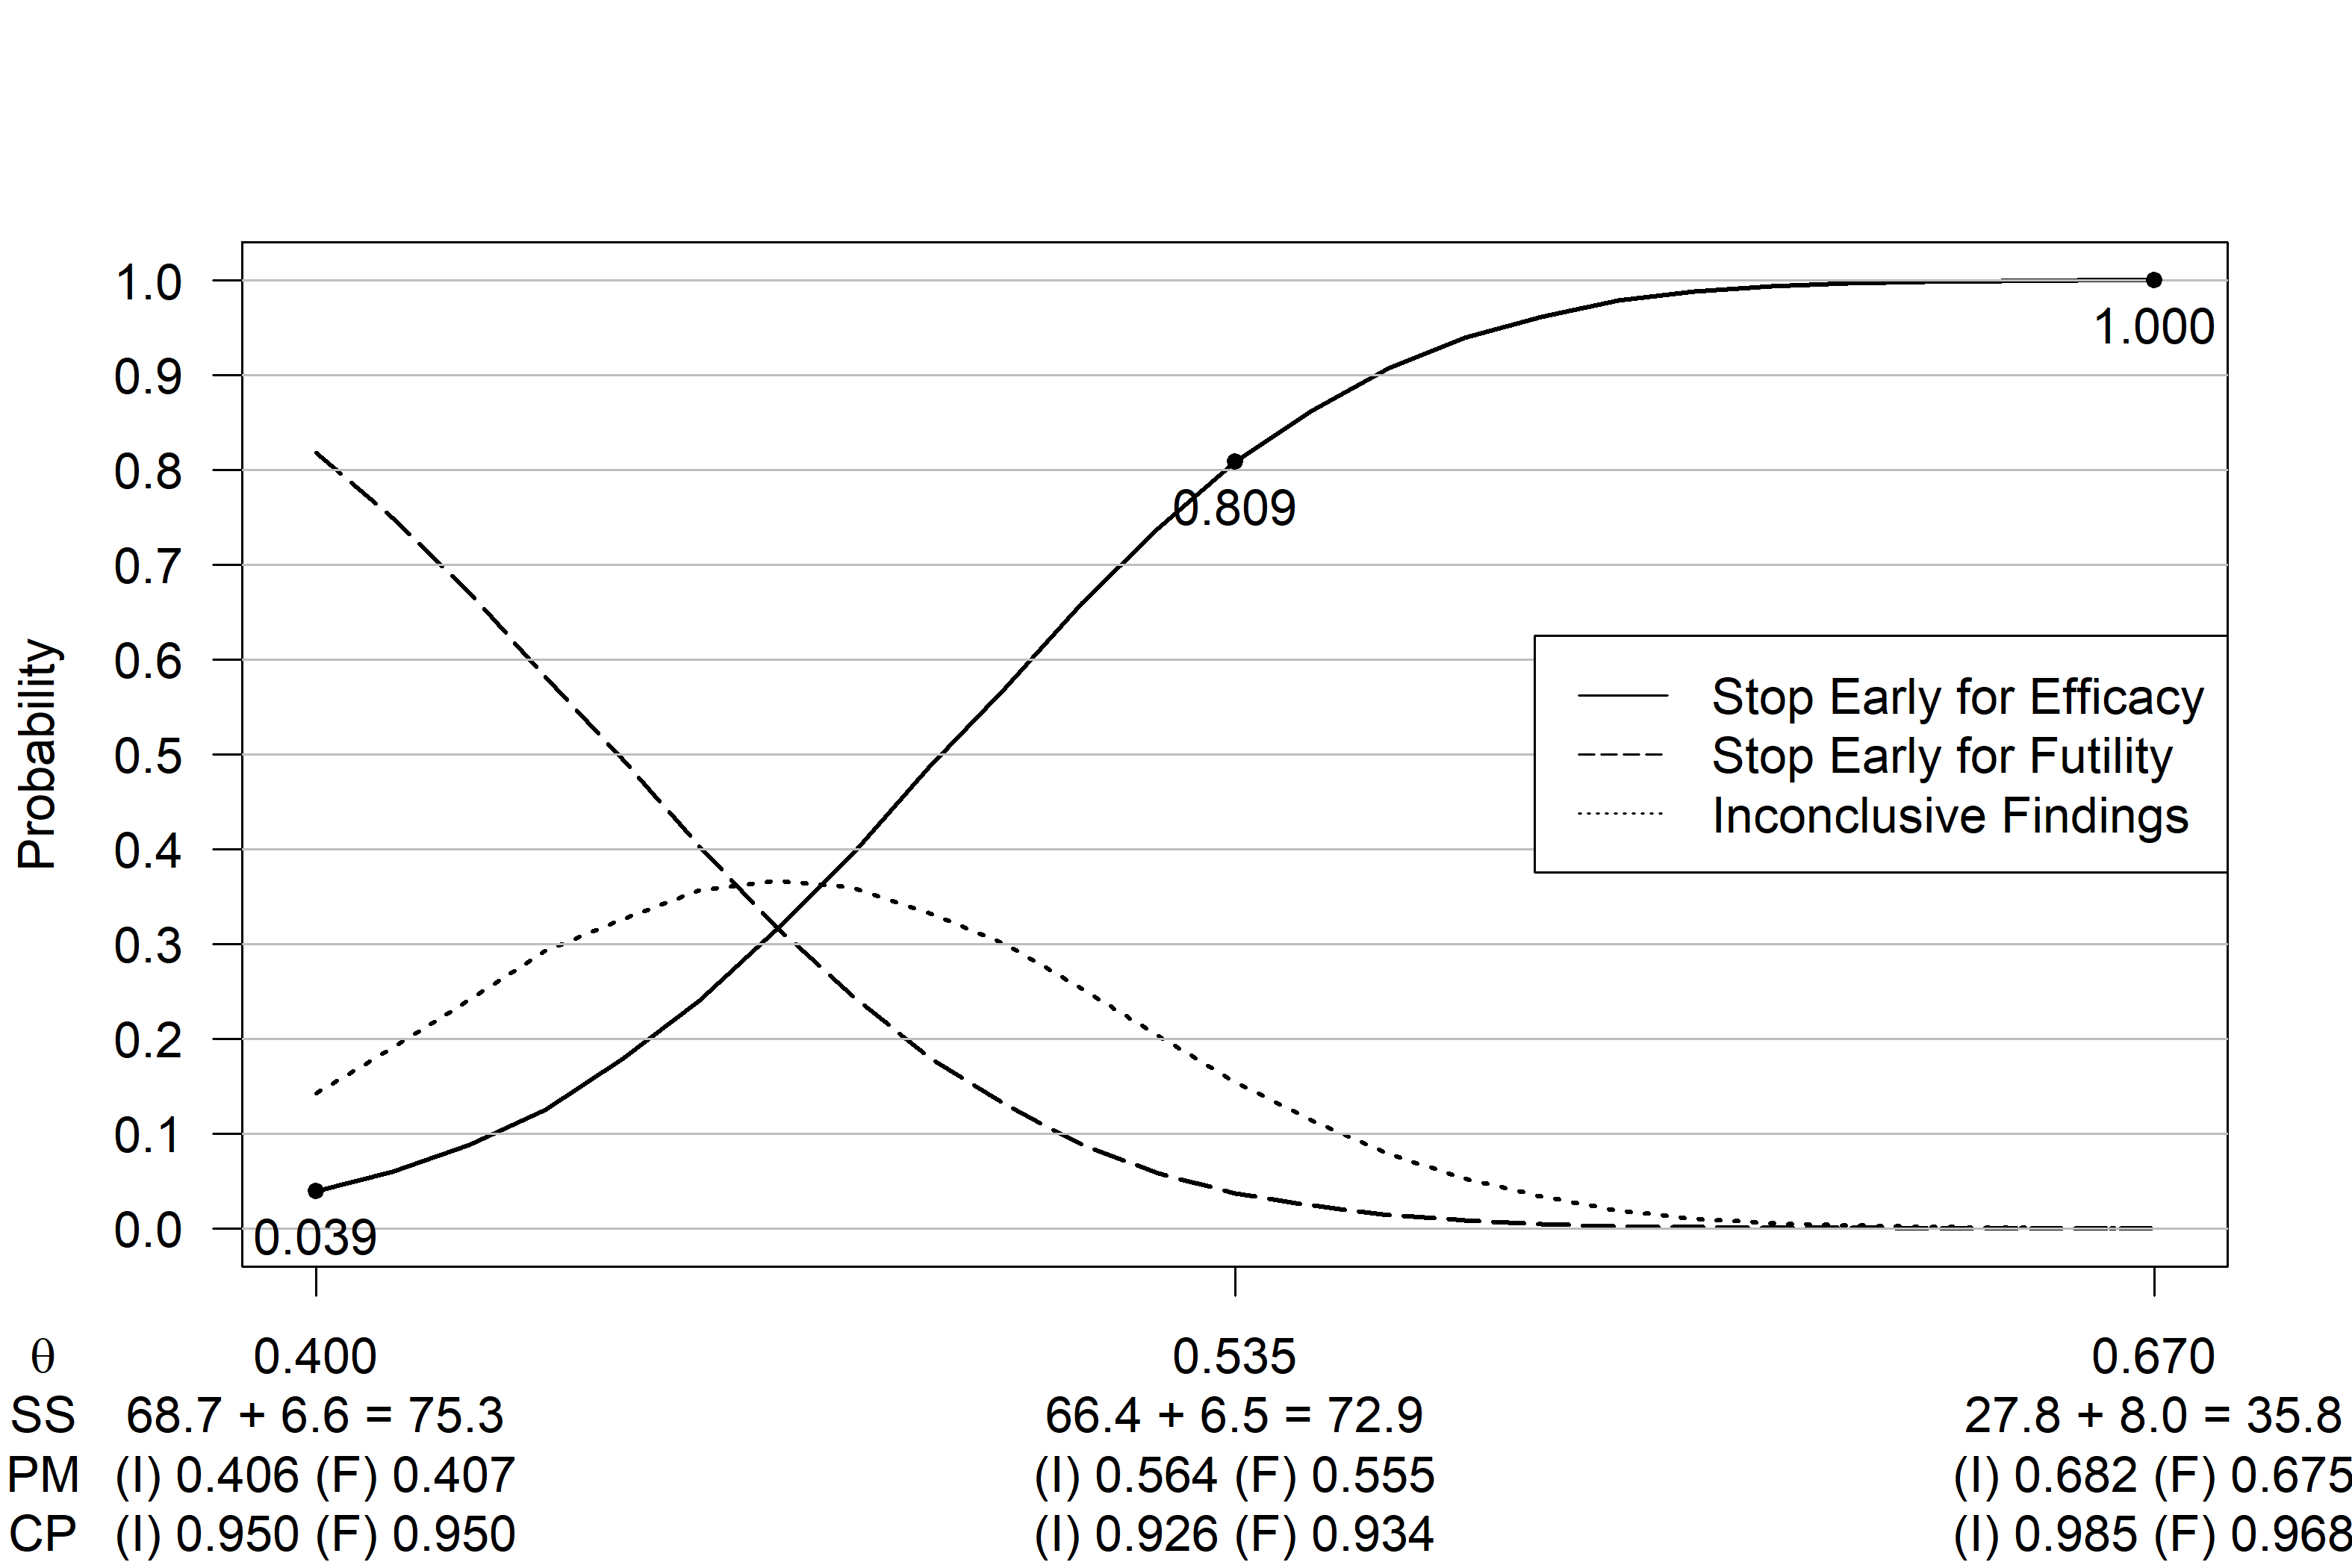
\includegraphics[width=6in]{figureS2b.png}
 \caption{Modification of enthusiastic prior parameterization in Example \ref{sec:example1}. A, default enthusiastic prior (Figure \ref{fig:figure1}(c)). B, flattened enthusiastic prior (Figure \ref{fig:figure1}(d)). Both designs use concentrated skeptical prior (Figure \ref{fig:figure1}(b)).}
\label{fig:robustness1}
\end{center}
\end{figure}
\begin{figure}\begin{center}

 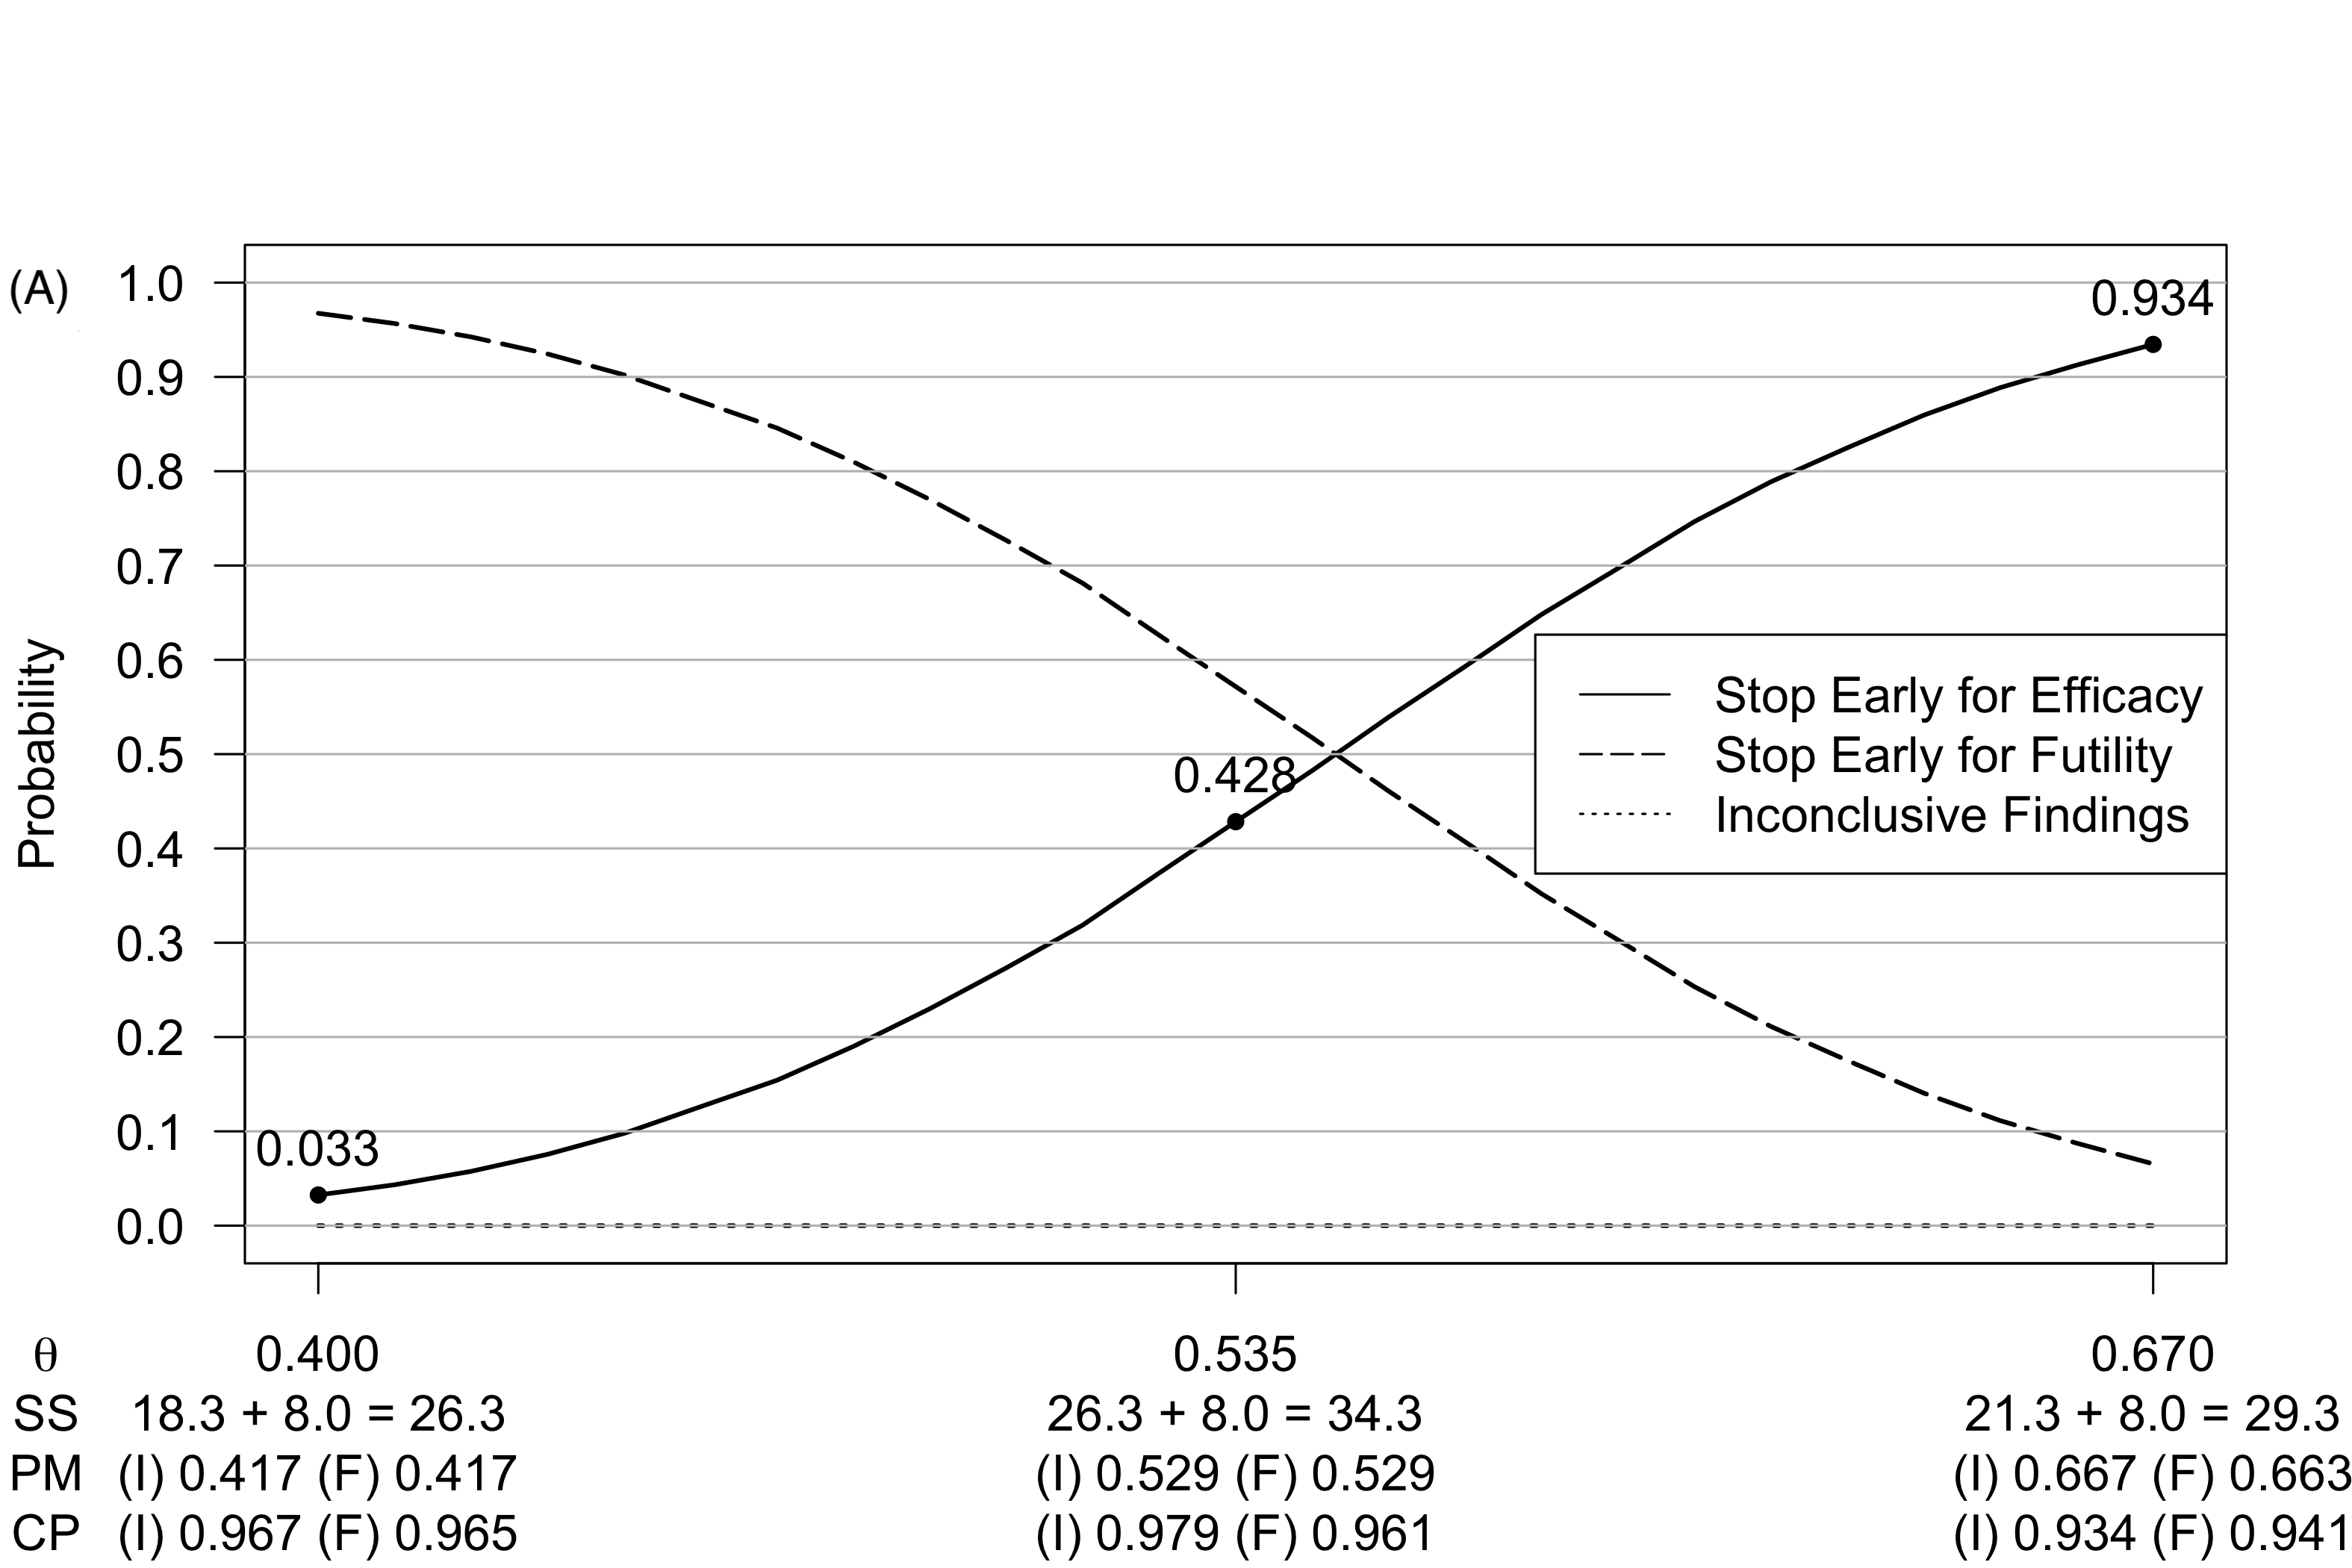
\includegraphics[width=6in]{figureS2c.png}
 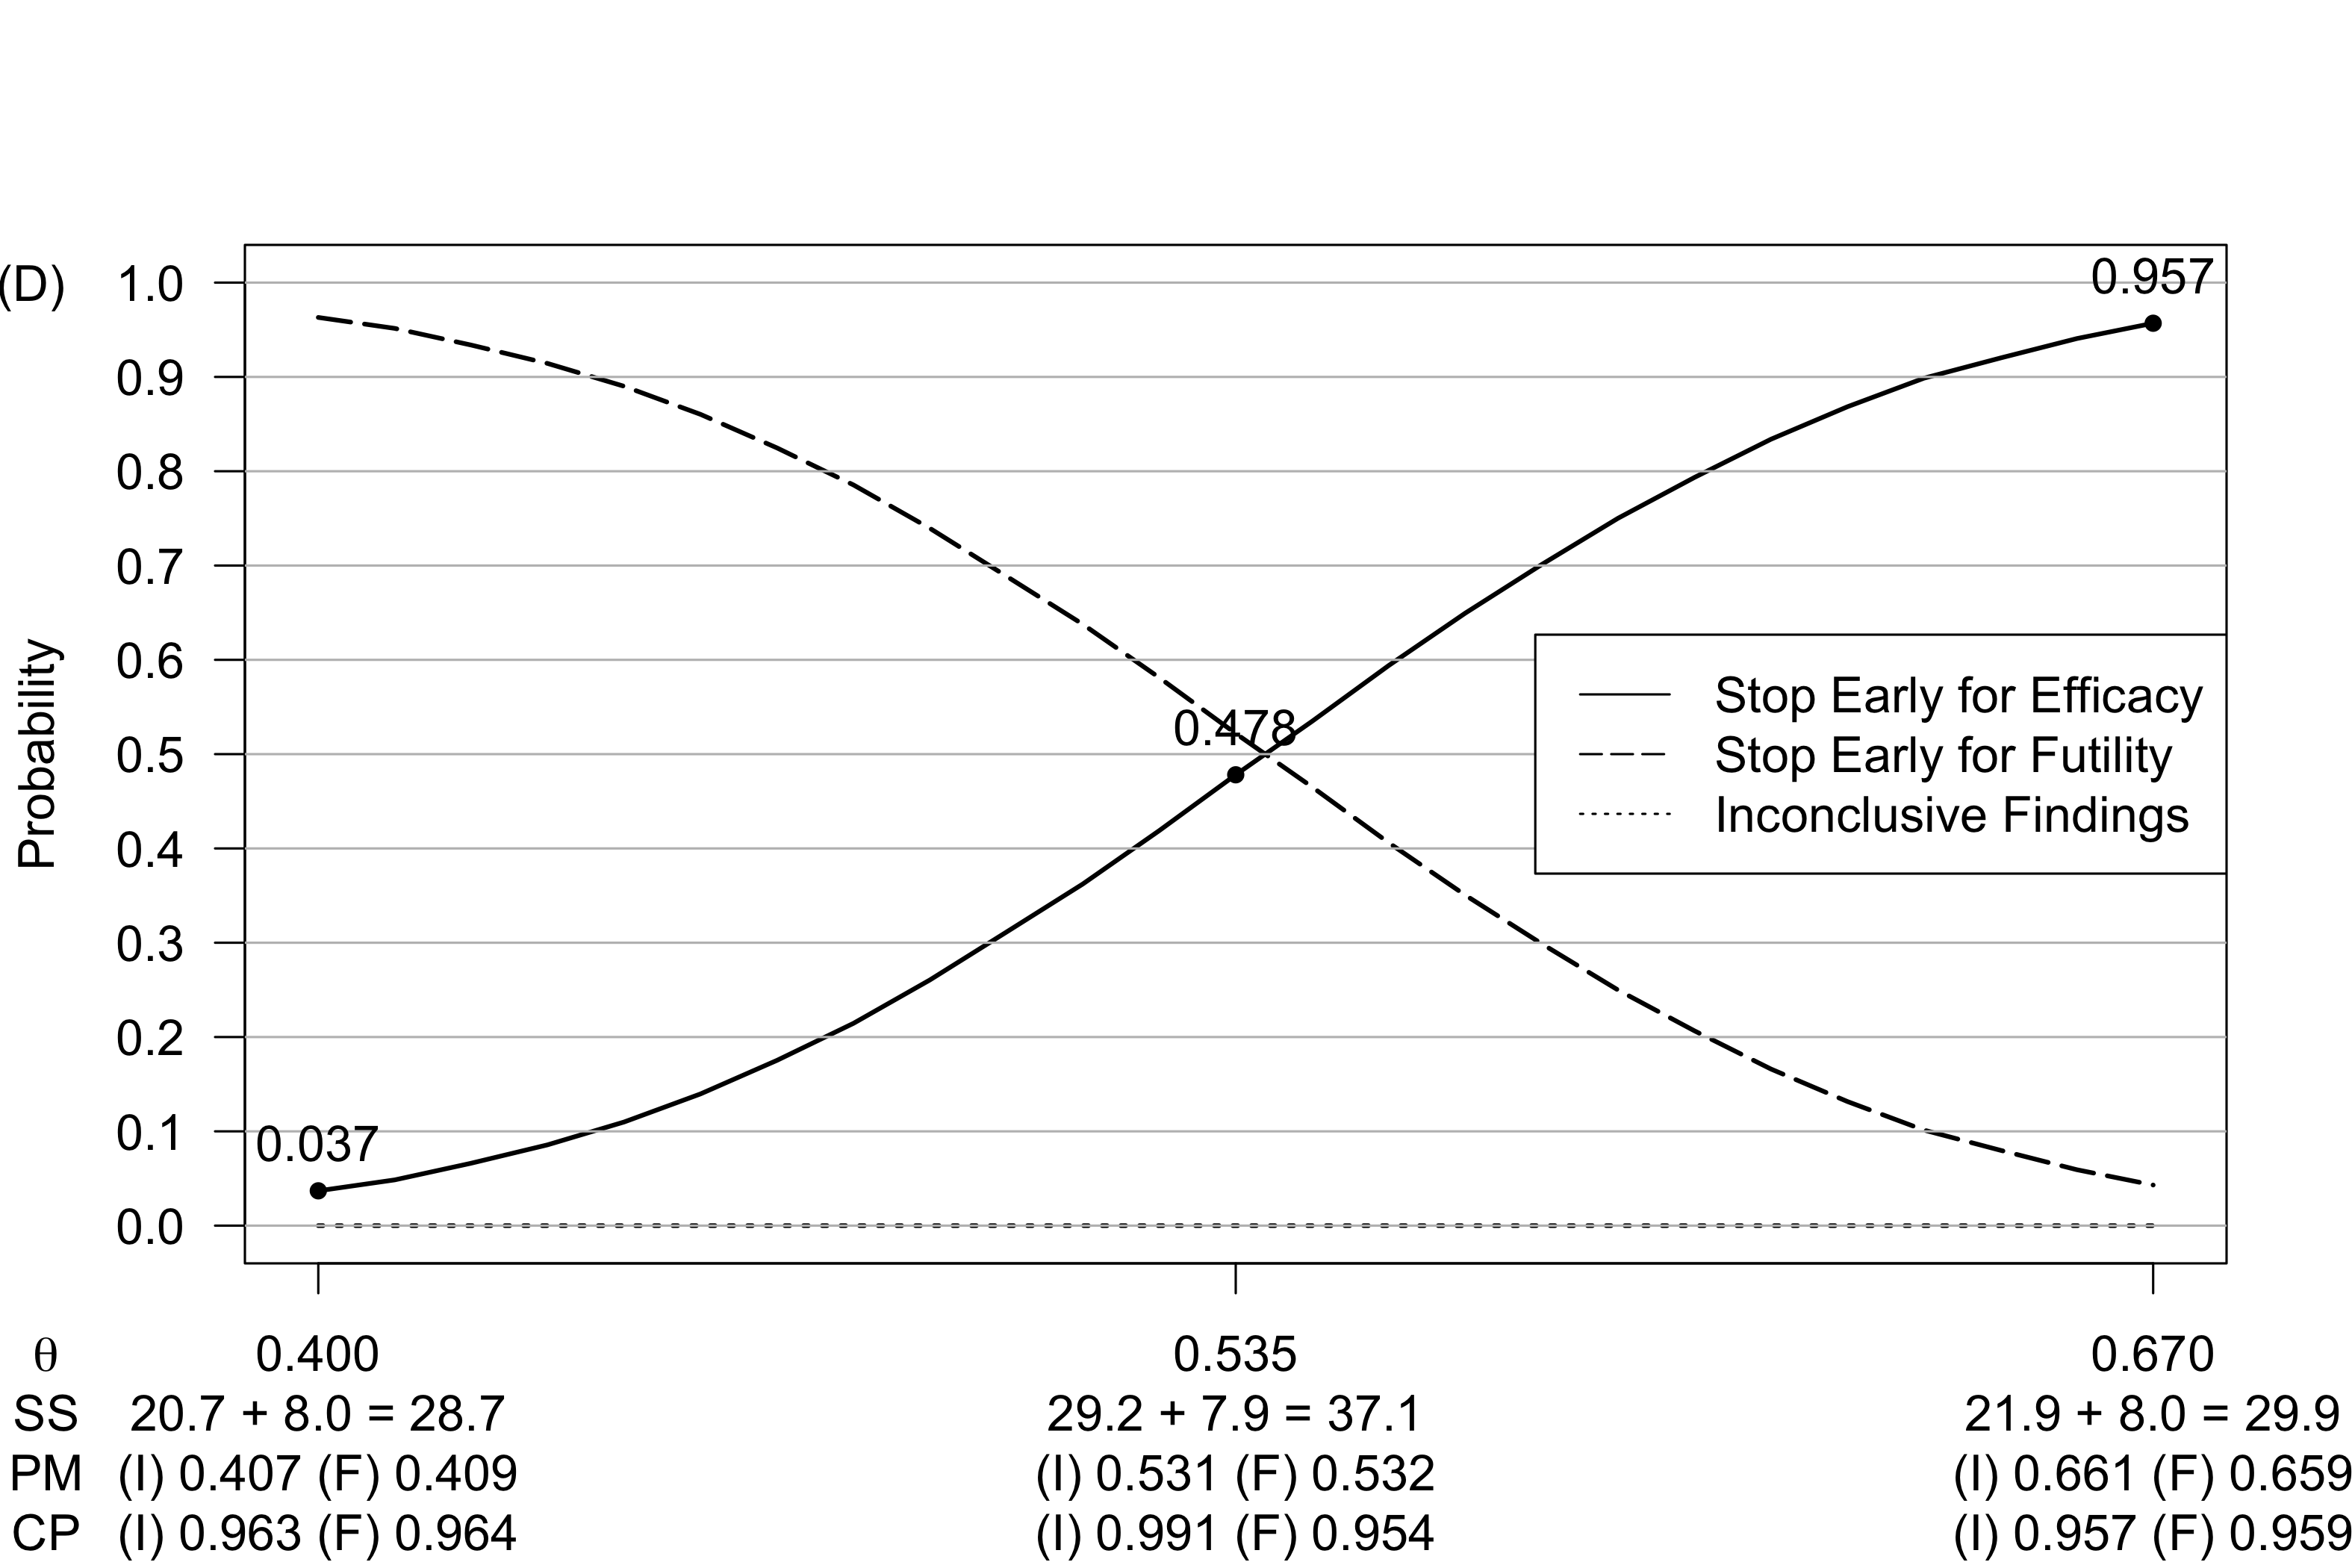
\includegraphics[width=6in]{figureS2d.png}
 \caption{Modification of enthusiastic prior parameterization in Example \ref{sec:example1}. A, default enthusiastic prior (Figure \ref{fig:figure1}(c)). B, flattened enthusiastic prior (Figure \ref{fig:figure1}(d)). Both designs use default skeptical prior (Figure \ref{fig:figure1}(a)).}
\label{fig:robustness2}
\end{center}
\end{figure}

%% latex table generated in R 4.0.0 by xtable 1.8-4 package
% Tue Jul 14 12:05:34 2020
\begin{table}[ht]
\centering
\begin{tabular}{llrrrr}
  \hline
  \hline
0.4 & FUT INITIAL & 0.7572 & 0.7653 & 0.8069 & 0.8183 \\ 
   & FUT FINAL & 0.5862 & 0.5930 & 0.6371 & 0.6455 \\ 
   & SS & 71.0198 & 73.0444 & 66.6849 & 68.6982 \\ 
  0.535 & FUT INITIAL & 0.0260 & 0.0251 & 0.0384 & 0.0370 \\ 
   & FUT FINAL & 0.0137 & 0.0127 & 0.0199 & 0.0193 \\ 
   & SS & 56.8978 & 66.8005 & 56.1953 & 66.4028 \\ 
  0.67 & FUT INITIAL & 0.0000 & 0.0000 & 0.0000 & 0.0000 \\ 
   & FUT FINAL & 0.0000 & 0.0000 & 0.0000 & 0.0000 \\ 
   & SS & 22.9456 & 27.8308 & 23.0299 & 27.8094 \\ 
   \hline
\end{tabular}
\end{table}


\label{lastpage}

\end{document}